\documentclass{article}
\usepackage{amsmath}
\usepackage{amssymb}
\usepackage{enumitem}
\usepackage{algorithm}
\usepackage{listings}
\usepackage{color,xcolor}
\usepackage[T1]{fontenc}
\usepackage{etoolbox}
\usepackage{multicol}
\usepackage{geometry}
\usepackage{tikz, pgfplots, tkz-euclide,calc}
    \usetikzlibrary{patterns,snakes,shapes.arrows,3d}
    \geometry{
        total = {160mm, 237mm},
        left = 25mm,
        right = 35mm,
        top = 30mm,
        bottom = 30mm,
      }

\newcommand{\enter}{\raisebox{-1.8pt}{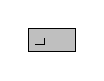
\begin{tikzpicture}[scale=0.3]
    \draw[thin,fill=lightgray] (0,0) rectangle (2,1);
    \draw (0.3,0.3) -- (0.7,0.3)--(0.7,0.6);     
\end{tikzpicture}}}

\definecolor{pgray}{rgb}{0.5,0.5,0.5}
\definecolor{pblue}{rgb}{0.13,0.13,1}
\definecolor{pgreen}{rgb}{0,0.5,0}
\definecolor{pred}{rgb}{0.9,0,0}
\definecolor{pgrey}{rgb}{0.46,0.45,0.48}
\definecolor{pcyan}{HTML}{D4EFFC}
\definecolor{lblue}{HTML}{00AEEF}
\definecolor{input}{HTML}{AAE1FA}
\definecolor{bg}{rgb}{0.95, 0.95, 0.92}
\definecolor{vscode}{HTML}{282A36}

\newcommand{\nextline}[1]{\raisebox{0pt}[1pt]{\colorbox{input}{#1}}}

\usepackage{listings}

\lstdefinestyle{Liang}{language=Java,
showspaces=false,
showtabs=false,
breaklines=true,
showstringspaces=false,
breakatwhitespace=true,
commentstyle=\color{pgray},
keywordstyle=\color{pblue},
stringstyle=\color{pgreen},
basicstyle=\small\ttfamily,
frame=single,
backgroundcolor=\color{pcyan},
escapeinside={(*}{*)},}

\lstdefinestyle{output}{
    language=Java,
    backgroundcolor=\color{vscode},
    basicstyle=\small\ttfamily\color{white},
    frame=single,
    escapeinside={(*}{*)},
    showspaces=false,
    showtabs=false,
    breaklines=true,
    showstringspaces=false,
    breakatwhitespace=true,
    }

\lstdefinestyle{standard}{language=Java,
    showspaces=false,
    showtabs=false,
    breaklines=true,
    showstringspaces=false,
    breakatwhitespace=true,
    commentstyle=\color{pgray},
    keywordstyle=\color{pblue},
    stringstyle=\color{pgreen},
    basicstyle=\small\ttfamily,
    frame=single,
    backgroundcolor=\color{bg},
    escapeinside={(*}{*)},}

\lstset{style=Liang}

\title{\textbf{Week 1 Assigment}}
\date{9 September 2024}
\author{Teosofi H.A \& Hafidz M.}

\begin{document}
    \maketitle
    \pagenumbering{gobble}
    \section*{Tugas Mandiri}
    \begin{enumerate}
        \item Buatlah program yang outputnya menampilkan nama panggilan anda dengan ketentuan
        \begin{itemize}
            \item Setiap huruf karakter pada nama anda akan dikontruksi oleh huruf itu sendiri
            \item Gunakan \texttt{\color{lblue}System.out.println()} untuk membuat setiap baris
            \item Minimal baris output yang dihasilkan adalah 5
        \end{itemize}
        Contoh Output:
        \begin{enumerate}[label=(\arabic*)]
            \item Nama Panggilan : Teo
            \begin{lstlisting}[style=output]
Nama : Teosofi Hidayah Agung

TTTTTTTT  EEEEE      OOO  
   TT     E        OO   OO
   TT     EEEEE   O       O
   TT     E        OO   OO
   TT     EEEEE      OOO
            \end{lstlisting}
            \item Nama Panggilan : Hafidz
            \begin{lstlisting}[style=output]
Nama : Hafidz Mulia

HH  HH      A        FFFFF   II   DDDD    ZZZZZ
HH  HH     A A       F       II   D   D      Z
HHHHHH    AAAAA      FFF     II   D   D     Z
HH  HH   A     A     F       II   D   D    Z
HH  HH  A       A    F       II   DDDD    ZZZZZ
            \end{lstlisting}
        \end{enumerate}
        
        
        \item Sebutkan dan jelaskan kesalahan apa saja yang kamu temukan pada potongan program java berikut, kemudian perbaiki program tersebut.
        \begin{lstlisting}[style=standard]
public class Kelompok1 {
    public static void main(String[] args) {
        System.out.println(Halo, nama ku Balmond);
        System.out.println("Hello World"+12)
        a=100;
    }
        \end{lstlisting}

    \end{enumerate}
\end{document}